\documentclass[conference]{IEEEtran}
\usepackage{cite}
\usepackage{graphicx}
\usepackage{booktabs}
\usepackage{amsmath}
\usepackage{url}
\usepackage[hidelinks]{hyperref}
\usepackage{tikz}
\usetikzlibrary{shapes.geometric,arrows.meta,positioning,fit,backgrounds}
\setlength{\textfloatsep}{14pt plus 3pt minus 3pt}
\setlength{\floatsep}{14pt plus 3pt minus 3pt}
\setlength{\intextsep}{14pt plus 3pt minus 3pt}

\begin{document}

\title{AC-RAG: Evidence-Driven Adaptive Retrieval-Augmented Generation with Control-Step Budgeting}

\author{
\IEEEauthorblockN{
S. Suryanarayana Raju\IEEEauthorrefmark{1},
Mullapudi Sai Nikhil\IEEEauthorrefmark{1},
Pasam Venkata Brahmendra\IEEEauthorrefmark{1},\\
Mandadapu Lokesh\IEEEauthorrefmark{1},
Medicharla Adi V Narasimha Sai Krishna\IEEEauthorrefmark{1},
Obulapuram Sai\IEEEauthorrefmark{1}
}
\IEEEauthorblockA{
\IEEEauthorrefmark{1}Department of Information Technology,
Sagi Rama Krishnam Raju Engineering College (Autonomous),\\
Bhimavaram -- 534202, Andhra Pradesh, India\\
sainikhilmullapudi1604@gmail.com,
pasamvenkatabrahmendra@gmail.com,
lokeshmandadapu96@gmail.com,\\
aadimedicharla44@gmail.com,
saiobulapuram9112@gmail.com
}
}

\maketitle

\begin{abstract}
Most RAG systems retrieve a fixed number of passages, generate once, and stop. If
the evidence was incomplete, nothing downstream notices. AC-RAG is our attempt to
fix that: a LangGraph pipeline that breaks a query into explicit evidence
requirements, checks what was retrieved against those requirements, re-retrieves
the missing pieces, and verifies every generated claim against the retrieved text
before deciding to answer or abstain, all under a fixed control-step budget. We
tested it against a naive single-pass baseline on 120 questions over a technical
paper, across eight ablation configurations. The headline result surprised us: the
full pipeline does not beat the baseline on aggregate composite quality (0.483 vs.
0.492), and it is far slower (20.6s vs. 8.5s per query) and more expensive to run.
It does win on faithfulness (0.448 vs. 0.444), and, more usefully, it fails in ways
we can actually diagnose. Digging into the results, five questions (4\% of the set)
account for most of the composite gap, and in every one of them the pipeline had
already retrieved and validated the right evidence; the generator and critic simply
abstained anyway. Drop those five and AC-RAG wins on the remaining 115. We ran a
full per-component ablation (planner, validator, context refiner, critic removed
one at a time, plus retrieval width) to pin down which parts drive the faithfulness
gain and which drive the false abstentions, and along the way we found and fixed a
router defect that let repair loops run up to 4$\times$ past their intended budget.
We also tested three small, hand-written probe sets at different difficulty levels
and found AC-RAG's advantage is not uniform; it depends on the kind of question
being asked. Our conclusion is correspondingly narrow: evidence-driven control
genuinely helps faithfulness and failure diagnosability, it is not yet a uniform
win over naive RAG, and the fix is probably selective activation rather than
running the full pipeline on everything, which we lay out as future work.
\end{abstract}

\begin{IEEEkeywords}
retrieval-augmented generation, LLM self-reflection, claim verification, adaptive
retrieval, control-step budgeting, LangGraph, agentic RAG
\end{IEEEkeywords}

\section{Introduction}

Retrieval-augmented language models ground generation in external documents and cut
down on hallucination relative to closed-book generation \cite{lewis2020rag}. The
standard pipeline, though, is mostly static. Embed the query, pull the top-$k$
passages by similarity, generate an answer in one pass. Nothing in that loop ever
notices if the evidence turns out insufficient, contradictory, or only loosely related
to what was actually asked. A short factual question might need exactly one passage.
A question that combines several facts, or spans multiple sections of a document,
needs evidence pulled together from different parts of the collection. Retrieve too
little and the answer has gaps. Retrieve too much and you add material that does not
help, material a downstream verification step now has to sort through.

Good retrieval does not guarantee a correct answer either. A passage can be topically
on-target and still fail to support the specific claim the model goes on to make. This
is what has driven a growing body of work on factuality, iterative retrieval, agentic
reasoning, and self-reflection
\cite{maynez2020faithfulness,kryscinski2020factcc,pagnoni2021frank,yao2023react,shinn2023reflexion,singh2025agenticrag,li2025ragreasoning}.
Recent systems increasingly build evidence sufficiency and failure recovery into the
pipeline itself, rather than hoping a single forward pass gets it right. Several lines
of work add a reflection or correction loop around the basic retrieve-generate setup,
letting the model re-retrieve or revise its answer when the first attempt is judged
inadequate (Self-RAG \cite{selfrag}, Corrective RAG \cite{crag}, CtrlA
\cite{liu2025ctrla}). These approaches trade latency and inference cost for quality,
on the assumption that the trade is worth it. That assumption rarely gets
stress-tested against a naive baseline on a controlled, non-cherry-picked question set
with full failure-mode logging. Most reported evaluations give an aggregate quality
delta and stop there, with no forensic breakdown of which questions got worse, why, or
whether the degradation is spread thin across the set or concentrated in a handful of
pathological cases.

This paper is about AC-RAG (Adaptive Control RAG), a LangGraph pipeline that makes
that reflection loop explicit and bounded. Before retrieval, a query analyzer breaks
the question into typed \emph{evidence requirements} (a numeric value, a procedural
description, a comparison between two entities), each carrying an expected modality
and a priority. After retrieval, a validator scores what came back against each
requirement and computes a coverage score. If coverage on a high-priority requirement
is insufficient, a targeted re-retrieval round fires instead of moving straight to
generation. After generation, extracted claims get checked against the retrieved
context, and a critic scores the answer on five dimensions, triggering a repair
(regeneration, targeted re-retrieval, or re-planning) when it fails. All of this
looping is bounded by an explicit control-step budget
(\texttt{MAX\_TOTAL\_CONTROL\_STEPS}), so the system is guaranteed to stop: with an
accepted answer, an explicit abstention, or an explicit ``max retries exhausted''
failure that is itself a loggable, analyzable event, not a silent low-quality answer
that looks indistinguishable from a confident correct one.

We are not claiming this architecture beats naive RAG outright. What we have is an
honest, fully instrumented comparison. We show where the architecture helps, where it
actively hurts, why, and what specific code-level defect accounted for part of the
measured cost, a defect we found and fixed mid-study and report in full, because it
illustrates exactly the kind of failure a bounded-but-incompletely-enforced control
loop can hide. Four contributions, concretely: (1) a LangGraph implementation of
evidence-driven adaptive RAG with an explicit, globally bounded control-step budget;
(2) a non-cherry-picked, positionally-ordered 120-question evaluation with a full
eight-configuration ablation, logged per-query in enough detail to trace every failure
to a specific stage and reason; (3) a forensic analysis identifying \emph{false
abstention}, the model refusing to answer despite having retrieved and validated the
right evidence, as the dominant driver of the aggregate quality gap, not a broad
quality deficit; and (4) a question-type sensitivity analysis showing the
architecture's net value is conditional, not uniform.

The rest of the paper: Section~\ref{sec:related} surveys related work in RAG, agentic
retrieval, and RAG evaluation. Section~\ref{sec:problem} states the problem formally.
Section~\ref{sec:architecture} walks through the AC-RAG pipeline. Section~\ref{sec:setup}
covers the evaluation setup. Section~\ref{sec:results} reports results: the headline
comparison, the full ablation, the forensic false-abstention analysis, and the
question-type sensitivity probes. Section~\ref{sec:discussion} discusses what these
results mean for deploying this class of architecture. Section~\ref{sec:limitations}
states limitations plainly, and Section~\ref{sec:conclusion} closes with directions
for future work.

\section{Related Work}
\label{sec:related}

\textbf{Retrieval-Augmented Generation.} The original RAG formulation
\cite{lewis2020rag} combines a dense retriever with a seq2seq generator in one forward
pass. Dense Passage Retrieval \cite{karpukhin2020dpr} and Fusion-in-Decoder
\cite{izacard2021fid} improved semantic retrieval and multi-passage combination
respectively, but both treat retrieval as a single, non-adaptive step: a fixed $k$
passages, retrieved once, regardless of how hard the query is or whether the evidence
was actually enough.

\textbf{Agentic reasoning and self-reflection.} Agent-based reasoning brought a
different kind of control over generation. ReAct \cite{yao2023react} interleaves
reasoning with tool use, retrieval included, while Reflexion \cite{shinn2023reflexion}
studies iterative feedback across attempts at a task, so the model can decide at
inference time whether it needs another piece of evidence or another try. Broader
surveys group \emph{Agentic RAG} and \emph{RAG-reasoning} as systems that combine
planning, reflection, tool use, and iterative retrieval
\cite{singh2025agenticrag,li2025ragreasoning,mishra2026sokagentic}.

\textbf{Self-reflective and corrective RAG.} Self-RAG \cite{selfrag} trains a model to
emit reflection tokens deciding whether to retrieve at all, and to critique its own
output after the fact. Corrective RAG \cite{crag} adds a lightweight retrieval
evaluator that falls back to web search when the retrieved documents look irrelevant.
Both report gains over static RAG baselines, but neither gives a latency/cost-controlled
comparison with a full ablation of which sub-component actually drives the
improvement, and neither reports a forensic breakdown of what still fails once the
proposed mechanism is in place.

\textbf{Adaptive retrieval.} A different line of work asks a narrower question: how
much retrieval does a given query actually need? Moskvoretskii et al.\ look at
retrieval adaptation under model uncertainty, weighing answer quality against
inference efficiency directly \cite{moskvoretskii2025adaptive}. CtrlA
\cite{liu2025ctrla} decides when and how to invoke retrieval using internal model
signals rather than an external evaluator. RAG+ \cite{wang2025ragplus} studies
application-aware reasoning over retrieved evidence. AC-RAG sits in this line of work
too, letting retrieval depth, strategy, and lexical/dense weighting vary per query, but
uses an explicit evidence-coverage signal rather than model uncertainty alone to decide
whether another retrieval round is needed.

\textbf{Claim verification and hallucination detection.} A separate body of work
studies faithfulness and factual consistency relative to source material
\cite{maynez2020faithfulness,kryscinski2020factcc,pagnoni2021frank}, usually by
breaking generated text into atomic claims and checking each against the source.
AC-RAG uses this same decomposition, but as an \emph{internal control signal}: an
unsupported or contradicted claim fires a repair loop inside the pipeline itself,
rather than only showing up as a post-hoc evaluation metric after generation is
already final.

\textbf{Evidence-sufficiency-driven retrieval and failure repair.} Two recent systems
are closest to this work in spirit: both make evidence sufficiency and failure repair
explicit parts of an agentic RAG loop. AdaKG-RAG \cite{yuan2026adakg} runs a
hypothesis-and-verification loop over a knowledge graph to spot incomplete evidence and
search for the missing bridge facts in multi-hop QA. Doctor-RAG \cite{jiao2026doctorrag}
instead locates the earliest failure point in an agentic trajectory and repairs only
that part, reusing whatever was already validated instead of starting over. AC-RAG
tackles a similar problem, evidence sufficiency and reason-specific repair, through
query-derived typed evidence requirements, requirement-level coverage checks, and
targeted re-retrieval, but with no knowledge graph, and without AdaKG-RAG's or
Doctor-RAG's finer-grained prefix reuse or earliest-failure localization. Different
failure reasons in AC-RAG do route to different repair actions (targeted retrieval,
regeneration, re-planning), but the pipeline still redoes already-validated work when a
late-stage failure is detected.

\textbf{RAG evaluation.} Evaluation methodology has moved past a single aggregate
accuracy number too. RAGAS \cite{es2024ragas} proposes automated, reference-free
metrics for faithfulness and relevance. RAGChecker \cite{ru2024ragchecker} separates
retrieval quality from generation quality for fine-grained diagnostics, and CRUX
\cite{ju2025crux} checks whether retrieved context actually covers what a long-form
answer needs. The common thread is reporting several complementary aspects of a RAG
system together instead of one score, which is why this paper reports faithfulness,
completeness, answer relevance, context utilisation, ROUGE-L, and a composite,
alongside latency, cost, error rate, and full per-query control-flow diagnostics.

Relative to this line of work, AC-RAG's contribution is mostly evaluative and
diagnostic, not purely architectural. That means a pre-registered, non-outcome-filtered
ablation across eight configurations; an explicit, globally bounded control-step
budget so reflection loops cannot silently inflate latency or cost without limit; full
per-query diagnostic logging that traces every failure to a specific pipeline stage and
reason; and a forensic analysis that separates a broad-based quality deficit from a
small number of pathological failure cases, a distinction most prior evaluations of
this class of system skip.

\section{Problem Definition}
\label{sec:problem}

Let $D$ denote a document collection and $q$ a user query. The standard RAG objective
is to produce an answer $a$ using evidence $R(q, D)$ retrieved from $D$:
\begin{equation}
a = \arg\max_a \; P(a \mid q, R(q, D))
\end{equation}
Here $R(q, D)$ is computed once, by a single fixed retrieval operation, and generation
has no way to signal back that it was not enough. A natural fix is to additionally
require the generated answer be faithful to its evidence, i.e.\
$\mathrm{Faith}(a, R(q, D)) \geq \tau$ for some acceptance threshold $\tau$, and to let
$R(q, D)$ be revised when that condition fails:
\begin{equation}
a^{*} = \arg\max_a \; P(a \mid q, R_t(q, D)) \;\; \text{s.t.}\;\; \mathrm{Faith}(a, R_t(q, D)) \geq \tau
\end{equation}
where $R_t$ is the evidence set after $t$ rounds of retrieval, bounded by a control-step
budget $T_{\max}$. AC-RAG implements this procedurally: the query analyzer decides what
$R(q, D)$ needs to contain (the evidence requirements), the validator checks whether
$R_t(q, D)$ currently satisfies those requirements, and the control loop either
increments $t$ (targeted retrieval) or repairs $a$ (regeneration) when it does not,
until the condition is met, the budget $T_{\max}$ runs out, or the system abstains. One
honest gap, flagged again in Section~\ref{sec:limitations}: in the actual
implementation, the acceptance gate is the critic's categorical five-dimension score,
not a direct numerical check against $\tau$. We state the intended formal objective
here and report that gap plainly rather than quietly papering over it.

\section{AC-RAG Architecture}
\label{sec:architecture}

AC-RAG is a directed graph of nodes over a shared state object, orchestrated with
LangGraph, routing conditionally between stages based on the current state.
Fig.~\ref{fig:retrieval-side} is the retrieval-side flow: the query becomes evidence
requirements, evidence gets retrieved, coverage is checked against those requirements,
and targeted retrieval fires if something important is still missing.
Fig.~\ref{fig:answer-side} is the answer-side flow: the generated response is broken
into claims, those claims are checked against the retrieved evidence, and a bounded
repair loop kicks in when a check fails, routing to targeted re-retrieval,
regeneration, or re-planning depending on why it failed.

\begin{figure}[t]
\centering
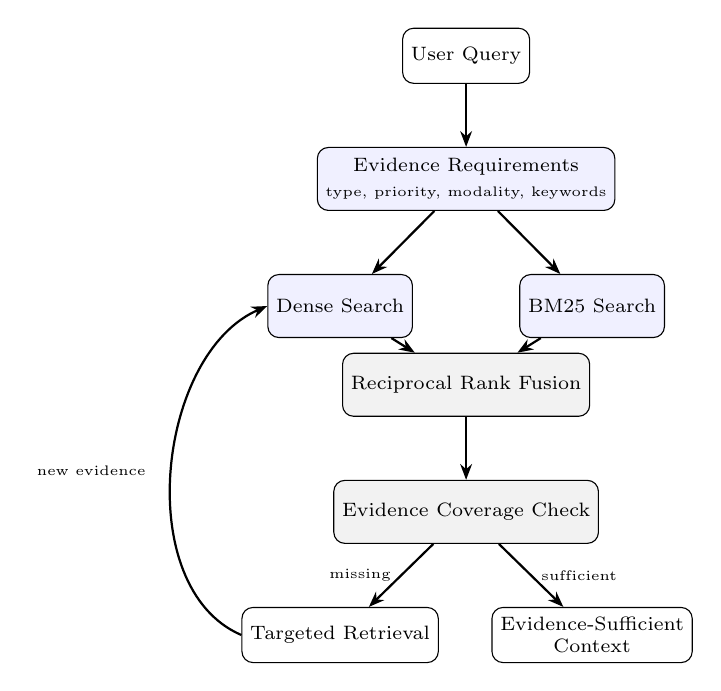
\begin{tikzpicture}[
  node distance=8mm and 8mm,
  box/.style={rectangle, draw, rounded corners, align=center, minimum height=8mm,
              font=\scriptsize, fill=blue!6, inner sep=3pt},
  decision/.style={rectangle, draw, rounded corners, align=center, minimum height=8mm,
                   font=\scriptsize, fill=gray!10, inner sep=3pt},
  term/.style={rectangle, draw, rounded corners, align=center, minimum height=7mm,
               font=\scriptsize, inner sep=3pt},
  arr/.style={-{Stealth[length=2mm]}, thick}
]
\node[term] (query) {User Query};
\node[box, below=of query] (req) {Evidence Requirements\\[1pt]\tiny type, priority, modality, keywords};
\node[box, below=of req, xshift=-16mm] (dense) {Dense Search};
\node[box, below=of req, xshift=16mm] (bm25) {BM25 Search};
\node[decision, below=18mm of req] (fuse) {Reciprocal Rank Fusion};
\node[decision, below=of fuse] (cov) {Evidence Coverage Check};
\node[term, below=of cov, xshift=-16mm] (targeted) {Targeted Retrieval};
\node[term, below=of cov, xshift=16mm] (suff) {Evidence-Sufficient\\Context};

\draw[arr] (query) -- (req);
\draw[arr] (req) -- (dense);
\draw[arr] (req) -- (bm25);
\draw[arr] (dense) -- (fuse);
\draw[arr] (bm25) -- (fuse);
\draw[arr] (fuse) -- (cov);
\draw[arr] (cov) -- node[left, font=\tiny] {missing} (targeted);
\draw[arr] (cov) -- node[right, font=\tiny] {sufficient} (suff);
\draw[arr] (targeted.west) .. controls +(-14mm,6mm) and +(-14mm,-6mm) .. node[left,font=\tiny,xshift=-2mm] {new evidence} (dense.west);
\end{tikzpicture}
\caption{Evidence-driven adaptive retrieval: query-derived requirements, hybrid
dense+lexical search with reciprocal rank fusion, requirement-level coverage checking,
and targeted re-retrieval on missing coverage.}
\label{fig:retrieval-side}
\end{figure}

\begin{figure}[t]
\centering
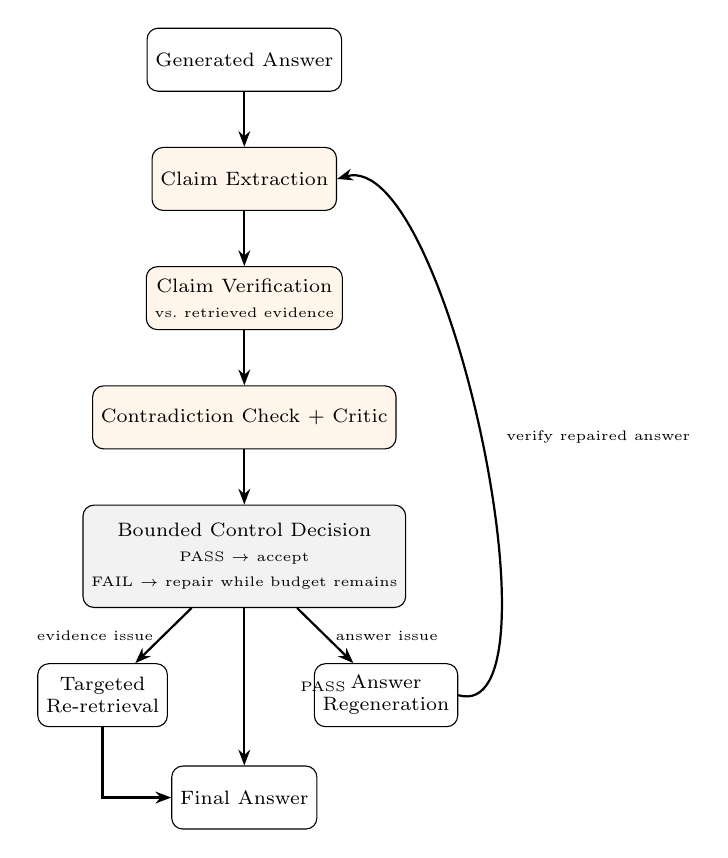
\begin{tikzpicture}[
  node distance=7mm and 8mm,
  box/.style={rectangle, draw, rounded corners, align=center, minimum height=8mm,
              font=\scriptsize, fill=orange!8, inner sep=3pt},
  decision/.style={rectangle, draw, rounded corners, align=center, minimum height=13mm,
                   font=\scriptsize, fill=gray!10, inner sep=3pt},
  term/.style={rectangle, draw, rounded corners, align=center, minimum height=8mm,
               font=\scriptsize, inner sep=3pt},
  arr/.style={-{Stealth[length=2mm]}, thick}
]
\node[term] (ans) {Generated Answer};
\node[box, below=of ans] (extract) {Claim Extraction};
\node[box, below=of extract] (verify) {Claim Verification\\[1pt]\tiny vs.\ retrieved evidence};
\node[box, below=of verify] (critic) {Contradiction Check + Critic};
\node[decision, below=of critic] (dec) {Bounded Control Decision\\[1pt]\tiny PASS $\to$ accept\\[1pt]\tiny FAIL $\to$ repair while budget remains};
\node[term, below=of dec, xshift=-18mm] (retr) {Targeted\\Re-retrieval};
\node[term, below=of dec, xshift=18mm] (regen) {Answer\\Regeneration};
\node[term, below=20mm of dec] (final) {Final Answer};

\draw[arr] (ans) -- (extract);
\draw[arr] (extract) -- (verify);
\draw[arr] (verify) -- (critic);
\draw[arr] (critic) -- (dec);
\draw[arr] (dec) -- node[left,font=\tiny] {evidence issue} (retr);
\draw[arr] (dec) -- node[right,font=\tiny] {answer issue} (regen);
\draw[arr] (dec) -- node[font=\tiny, xshift=10mm] {PASS} (final);
\draw[arr] (regen.east) .. controls +(14mm,-4mm) and +(14mm,4mm) .. node[right,font=\tiny,xshift=2mm] {verify repaired answer} (extract.east);
\draw[arr] (retr) |- (final);
\end{tikzpicture}
\caption{Claim-level verification and bounded repair: extracted claims are checked
against retrieved evidence and cross-checked for internal contradictions; the critic's
pass/fail decision routes to targeted re-retrieval, regeneration, or acceptance, bounded
by the remaining control-step budget.}
\label{fig:answer-side}
\end{figure}

\subsection{Pipeline stages}

The pipeline consists of the following stages, executed in order with conditional
back-edges for repair:

\begin{enumerate}
\item \textbf{Entry router}. First thing that touches the query. Decides whether it is
RAG-answerable or out of scope, before any retrieval runs. Cheap, but it saves real
retrieval cost on the queries the system should never have tried to answer from the
document collection in the first place.
\item \textbf{Query analyzer}. Breaks the query into sub-queries and a set of typed
\emph{evidence requirements}. Each one carries a \texttt{requirement\_type} (factual,
numeric, procedure, comparative, table, figure), an \texttt{expected\_modality}, a
priority (critical vs.\ normal), and retrieval keywords. Why bother? A single
query-passage similarity score gives the validator nothing concrete to check against;
typed requirements do.
\item \textbf{Retrieval planner}. Takes the query's complexity score and the evidence
requirements' types and turns them into a retrieval plan: top-$k$, MMR $\lambda$,
lexical/dense weighting, modality filter, depth. Numeric and value-lookup requirements
get a lexical-weight boost, since exact-match BM25 is what finds a specific number.
Procedural and conceptual requirements get a dense-weight boost instead, because the
right passage for a ``how/why'' question often shares almost no exact vocabulary with
the question itself.
\item \textbf{Retriever}. Runs hybrid retrieval, dense plus BM25, per the plan, and
fuses the two ranked lists with reciprocal rank fusion.
\item \textbf{Validator}. The workhorse of the design. It scores every retrieved
passage against every evidence requirement (semantic similarity, lexical overlap,
expected modality, exact-number signals where relevant), then computes a
per-requirement coverage score and an overall \texttt{evidence\_coverage}. Overall
coverage and coverage of \emph{critical} requirements are tracked separately on
purpose: a stack of generally relevant passages is worthless if the one essential fact
is still missing. When a critical requirement's coverage drops below a calibrated
threshold, it lands in \texttt{missing\_requirements} and triggers a targeted
re-retrieval round, searching specifically for that requirement's keywords rather than
just rerunning the original query.
\item \textbf{Context refiner}. Deduplicates retrieved passages by semantic similarity
to cut redundant context before generation. One protection matters here: any passage
that uniquely covers a keyword from an unmet evidence requirement is never dropped as
redundant, even if it looks topically similar to something already kept. Without that
rule, the refiner would happily throw away the one passage that actually answers a
sub-requirement in favor of a more generic look-alike.
\item \textbf{Generator}. Produces an answer with inline citations from the refined
context. The prompt is written to keep the response inside the supplied evidence and
discourage unsupported additions, but generation itself is never treated as the final
correctness check.
\item \textbf{Claim extractor / claim verifier / contradiction detector}. Breaks the
generated answer into atomic claims and checks each against the retrieved context. A
claim the generator itself labeled ``supported'' gets downgraded if its computed
support score falls below a threshold; a claim gets force-labeled ``contradicted'' if
its contradiction score exceeds a threshold, regardless of what label the generator
gave it. The same stage separately checks for contradictions between claims within the
same answer.
\item \textbf{Critic}. Scores the answer on five dimensions (1--5 scale). Three
outcomes: accept the answer, trigger a bounded repair (regeneration, targeted
re-retrieval, or query re-analysis, depending on the failure reason), or abstain when
evidence is still judged insufficient after repair attempts run out.
\end{enumerate}

\subsection{Control-step budgeting}

Every loop in the pipeline, retrieval re-rounds and generation repairs alike,
increments a shared \texttt{total\_control\_steps} counter. The router enforces three
bounds: a cap on retrieval rounds (\texttt{MAX\_RETRIEVAL\_ROUNDS} = 3), a cap on
generation repairs (\texttt{MAX\_GENERATION\_REPAIRS} = 2), and a global cap across all
loop types combined (\texttt{MAX\_TOTAL\_CONTROL\_STEPS} = 8). This guarantees
termination and makes the cost of ``trying harder'' explicit and bounded. Compare that
to self-reflection designs with no hard ceiling on repair attempts, where a
pathological case can in principle loop indefinitely, or until some unrelated external
timeout kills it.

We found a router defect during this evaluation, and it is worth describing in full.
The repair-cap check (\texttt{MAX\_GENERATION\_REPAIRS}) was only applied when the
critic's failure reason was \texttt{format} or the default \texttt{content} case. It
was not applied when the reason was \texttt{unsupported\_claim} or \texttt{coverage},
which happen to be the two most common failure reasons in practice. For those two, the
loop was gated only by the retrieval-round cap and the global step cap. Retrieval-round
count usually stayed well under its own cap of 3 while repair attempts kept climbing,
so \texttt{repair\_attempts} reached 7--8 on affected questions, nearly four times the
intended cap of 2, before the global ceiling of 8 finally stopped it. Per-query latency
on those questions went from an expected $\sim$20s to over 180s. The defect matters
beyond its direct performance hit: a control loop bounded in aggregate
(\texttt{MAX\_TOTAL\_CONTROL\_STEPS}) can still quietly blow through its own
more specific sub-budgets, and the aggregate bound alone does not prove each individual
loop type is behaving as designed. Every result in Section~\ref{sec:results} reflects
the corrected routing logic.

\section{Evaluation Setup}
\label{sec:setup}

\subsection{Corpus and test set}
\label{sec:corpus}

An earlier phase of this project used a 100-question subset that had been deliberately
pulled from a 150-question pool for questions where the full AC-RAG pipeline beat the
baseline. That was a selection-biased sample, and once we recognized it as one we threw
it out before any result in this paper. Everything reported here instead uses a fixed,
unbiased, positionally-ordered 120-question test set (ids 1--120, generated in a fixed
order and never filtered by outcome), built against ``Attention Is All You Need''
\cite{vaswani2017attention}. We chose a well-known, publicly available paper unrelated
to this project's own source material specifically to sidestep any authorship or
provenance concerns that would come from using the project's own prior report as its
own evaluation corpus. One limitation worth stating up front: the LLM doing generation
and scoring (GPT-4o-mini) was almost certainly exposed to this paper during
pretraining, which could inflate absolute faithfulness and composite scores for
\emph{both} baseline and AC-RAG equally. Since that confound is shared identically
across all eight configurations in this study, we treat the \emph{relative} comparison
between configurations as the signal that matters, and treat absolute score magnitudes
as weaker, not something to compare directly against scores from other systems on
other corpora. We also ran AC-RAG against a smaller, secondary SQuAD v2.0-derived
benchmark to check generalization beyond this single-document corpus; that result is
reported qualitatively in Section~\ref{sec:limitations} rather than as a primary
result, given its small sample size.

\subsection{Metrics}

Each generated answer $a$ is scored on five automated metrics against a reference
answer $a_{ref}$ and its retrieved context $C = \{c_1, \dots, c_n\}$.

\textbf{Faithfulness.} The answer is split into sentences $\{s_1,\dots,s_m\}$; each
sentence's grounding is its maximum cosine similarity to any retrieved passage, and
faithfulness is the mean over sentences:
\begin{equation}
\mathrm{Faith}(a, C) = \frac{1}{m}\sum_{i=1}^{m} \max_{c_j \in C} \cos\!\big(\mathrm{emb}(s_i), \mathrm{emb}(c_j)\big)
\end{equation}

\textbf{Answer relevance.} Cosine similarity between the query embedding and the full
answer embedding: $\mathrm{Rel}(q, a) = \cos(\mathrm{emb}(q), \mathrm{emb}(a))$.

\textbf{Context utilisation.} The fraction of retrieved passages actually cited in the
answer (via inline $[N]$ markers), falling back to a semantic-overlap count
(cosine similarity $>0.35$ to the full answer) when no citations are present:
\begin{equation}
\mathrm{CU}(a, C) = \frac{|\{c \in C : c \text{ is cited by or semantically present in } a\}|}{|C|}
\end{equation}

\textbf{ROUGE-L} is the standard longest-common-subsequence F1 between $a$ and
$a_{ref}$, and \textbf{completeness} is a model-judged coverage score of the reference
answer's required information content in $a$.

\textbf{Composite.} The five scores are combined by unweighted arithmetic mean:
\begin{equation}
\mathrm{Composite} = \tfrac{1}{5}\big(\mathrm{Faith} + \mathrm{Rel} + \mathrm{Comp} + \mathrm{CU} + \mathrm{ROUGE\text{-}L}\big)
\end{equation}

We did not touch any of these five formulas mid-study, on purpose, to avoid post-hoc
metric-shopping. Two known proxy-metric weaknesses are disclosed directly in
Section~\ref{sec:limitations} instead: $\mathrm{CU}$ mechanically penalizes a concise,
correctly-targeted answer that cites only a few of many retrieved passages, regardless
of whether the answer is right, and ROUGE-L penalizes a correct paraphrase of
$a_{ref}$.

\subsection{Configurations and hyperparameters}

Table~\ref{tab:params} lists the main pipeline hyperparameters for this evaluation. We
run eight configurations on the full 120-question set: \texttt{baseline\_rag} (naive
single-pass RAG, planner/validator/refiner/critic all disabled, leaving only retrieval
and generation), \texttt{full} (everything enabled), and six ablations each changing
exactly one component relative to \texttt{full}: \texttt{no\_planner} (rule-based
retrieval depth only, no LLM-refined plan), \texttt{no\_validator} (no coverage gating,
every retrieved passage passes through unfiltered), \texttt{no\_refiner} (no
deduplication, raw retrieved passages go straight to the generator), \texttt{no\_critic}
(no self-reflection loop, the first generated answer is always accepted),
\texttt{low\_k} (fixed $k=4$ regardless of query complexity), and \texttt{high\_k}
(fixed $k=12$ regardless of query complexity).

\begin{table}[t]
\centering
\caption{Pipeline hyperparameters for the N=120 evaluation}
\label{tab:params}
\begin{tabular}{ll}
\toprule
Parameter & Value \\
\midrule
Vector store & FAISS \\
Chunk size / overlap & 512 / 64 tokens \\
Retrieval range & $k = 4$ to $12$ \\
Retrieval method & Dense + BM25, RRF fusion \\
Evidence score threshold & 0.20 \\
Overall coverage threshold & 0.45 \\
Critical requirement coverage & 0.25 (recalibrated) \\
Maximum retrieval rounds & 3 \\
Maximum generation repairs & 2 \\
Maximum total control steps & 8 \\
Embedding model & text-embedding-3-large \\
Generation / evaluation model & GPT-4o-mini \\
Claim support threshold & 0.70 \\
\bottomrule
\end{tabular}
\end{table}

The critical-requirement coverage threshold got recalibrated during this study, from an
initially stricter 0.60 down to 0.25. We bypassed the stricter threshold on ten real
queries it had blocked and checked the resulting answers against ground-truth
references: 8 of 10 were correct despite validator scores as low as 0.33. That told us
the stricter threshold had no clean separation between genuinely insufficient and
genuinely sufficient evidence in that range. This was a disclosed, pre-registered
tuning decision made before the final evaluation runs, not something adjusted after
seeing final composite scores.

\section{Results}
\label{sec:results}

\subsection{Headline comparison: baseline vs.\ full, N=120}

Table~\ref{tab:headline} is the primary result. \texttt{full} improves faithfulness by
0.0045 over \texttt{baseline\_rag}, but it is worse on composite ($-0.0090$), answer
relevance ($-0.0108$), and context utilisation ($-0.0427$). It also racks up 11 outright
failures (``max retries exhausted'') against zero for the baseline, at 2.4$\times$ the
latency and roughly 1.9$\times$ the cost per query.

\begin{table}[t]
\centering
\caption{Headline comparison, N=120}
\label{tab:headline}
\begin{tabular}{lrr}
\toprule
Metric & baseline\_rag & full \\
\midrule
Faithfulness & 0.4437 & \textbf{0.4482} \\
Answer relevance & \textbf{0.6264} & 0.6156 \\
Completeness & 0.6783 & \textbf{0.6800} \\
Context utilisation & \textbf{0.2519} & 0.2092 \\
ROUGE-L & 0.4609 & \textbf{0.4631} \\
\textbf{Composite} & \textbf{0.4922} & 0.4832 \\
Errors (/120) & \textbf{0} & 11 \\
Avg.\ latency (s) & \textbf{8.51} & 20.56 \\
Avg.\ cost (USD/query) & \textbf{0.00147} & 0.00280 \\
\bottomrule
\end{tabular}
\end{table}

\subsection{Full ablation, N=120}

Table~\ref{tab:ablation} covers all eight configurations. \texttt{no\_critic} has the
lowest error rate of any non-baseline configuration (1/120), and a composite close to
\texttt{full}'s. That tells us the critic/self-reflection loop is the dominant source
of both abstentions and outright failures in the full pipeline, while contributing
comparatively little to the composite score itself. Most of the full pipeline's
composite is already recovered by retrieval, validation, and refinement alone, before
the self-reflection loop even runs. \texttt{no\_validator} and \texttt{no\_refiner}
both land close to \texttt{full} on composite but noticeably worse on faithfulness
(0.4326 and 0.4333 respectively, against 0.4482 for \texttt{full}), so the validator and
refiner are meaningfully suppressing hallucination even though neither moves the
headline composite much on its own. \texttt{high\_k} gets the highest faithfulness of
any configuration (0.5149), but also the highest error rate (20/120, 17\%) and the
highest cost: widening retrieval improves grounding when an answer succeeds, but it
sharply increases claim-verification failures too, and that eats most of the
faithfulness gain in aggregate. \texttt{low\_k} sits close to the baseline on composite
(0.4870) but is worse on faithfulness (0.4289), the lowest of any configuration.

\begin{table}[t]
\centering
\caption{Full ablation, N=120}
\label{tab:ablation}
\begin{tabular}{lrrrr}
\toprule
Config & Composite & Faith. & Errors & Cost (USD) \\
\midrule
baseline\_rag & \textbf{0.4922} & 0.4437 & \textbf{0} & 0.177 \\
full & 0.4832 & 0.4482 & 11 & 0.336 \\
no\_critic & 0.4851 & 0.4419 & \textbf{1} & 0.196 \\
no\_refiner & 0.4760 & 0.4333 & 11 & 0.251 \\
no\_validator & 0.4771 & 0.4326 & 12 & 0.286 \\
no\_planner & 0.4812 & 0.4324 & 13 & 0.302 \\
low\_k & 0.4870 & 0.4289 & 14 & 0.239 \\
high\_k & 0.4821 & \textbf{0.5149} & 20 & 0.421 \\
\bottomrule
\end{tabular}
\end{table}

\subsection{Forensic analysis: false abstentions drive the aggregate gap}

Of the 120 questions, 29 triggered an abstention (``the provided documents do not
contain sufficient information to answer this question'') under \texttt{full}. Five of
those are \emph{false} abstentions: retrieval and validation had already succeeded in
each case (4--8 passages retrieved and validated, evidence confidence $\geq$0.52), and
\texttt{baseline\_rag} answered the identical question correctly from the same corpus.
One example: ``What is the dropout rate used for the big model?'', which the baseline
answered correctly as $P_{drop}=0.1$, while \texttt{full} abstained despite the correct
passage sitting right there in its own validated context. These 5 cases alone account
for $-2.138$ of the total composite-delta sum of $-1.080$ across all 120 questions,
which means the remaining 115 questions actually sum to $+1.058$, a net
\emph{positive} delta for \texttt{full}. The headline result in Table~\ref{tab:headline}
being negative comes down to a handful of pathological false abstentions, not a
broad-based quality deficit across the set. This is the single most actionable finding
of the study: the failure is localized and specific, evidence correctly retrieved and
validated, generation/critic still refusing to use it, rather than diffuse across many
questions. That points to a targeted fix in the generator/critic interaction, not a
wholesale redesign of retrieval or validation.

\subsection{Query-complexity-dependent effects}

Splitting the 120-question set into complexity terciles by the query analyzer's own
complexity score, \texttt{full} underperforms \texttt{baseline\_rag} on low-complexity
queries (complexity $<0.4$, 79 questions, mean per-question composite delta
$-0.0155$), but outperforms it on mid-complexity queries (0.4--0.7, 41 questions, mean
delta $+0.0035$). That fits the architecture's intended use case: the control loop's
overhead is mostly wasted on trivial single-fact lookups, where one retrieval pass
already has the answer and extra validation/repair adds cost without adding
information. The machinery starts earning its keep as query complexity rises and a
single retrieval pass is less likely to be immediately sufficient.

We also probed this effect with four small, independently authored supplementary
five-question sets, each a separate baseline-vs.-full comparison, reported in
Table~\ref{tab:probes} as a qualitative signal rather than a statistically powered
result, given the small sample size. Taken together, the probes suggest the
architecture's net value depends on question type. It helps most on questions that
genuinely require synthesis or interpretation of a single concept, is neutral to mildly
negative on well-contained single-passage questions, and is close to a wash, small
faithfulness wins offset by cost and occasional errors, on questions that need evidence
assembled from multiple sections of the source document.

\begin{table}[t]
\centering
\caption{Question-type sensitivity probes (n=5 each, full vs.\ baseline)}
\label{tab:probes}
\begin{tabular}{lrrr}
\toprule
Probe type & $\Delta$Composite & $\Delta$Faith. & full errors \\
\midrule
Single-concept explanation & $+0.0121$ & $+0.0455$ & 1 \\
Single-section synthesis & $-0.1138$ & $-0.0399$ & 1 \\
Scattered multi-hop (set A) & $-0.0026$ & $+0.0052$ & 1 \\
Scattered multi-hop (set B) & $-0.0317$ & $-0.0355$ & 1 \\
\bottomrule
\end{tabular}
\end{table}

\section{Discussion}
\label{sec:discussion}

Put together, the headline result (Table~\ref{tab:headline}), the full ablation
(Table~\ref{tab:ablation}), and the forensic false-abstention analysis paint a more
specific picture than ``AC-RAG does/does not beat the baseline.''

The components do not contribute uniformly, and some of them actively trade
faithfulness against reliability. The critic/self-reflection loop causes most of the
full pipeline's abstentions and outright failures, removing it (\texttt{no\_critic})
drops the error rate from 11/120 to 1/120 while barely moving composite, yet it is also
the mechanism meant to catch unsupported claims in the first place. \texttt{high\_k}
shows the same tension from a different angle: wider retrieval produces the most
faithful individual answers in the study (0.5149) but also the highest failure rate.
More retrieved context just gives the claim verifier more surface area to find
something it judges unsupported, even when the underlying answer is correct. The
verification threshold seems conservative enough to reject a growing share of
genuinely correct answers as context size grows.

The false-abstention finding matters more than the headline composite gap it explains.
A false abstention happens when the system already did the hard part right, planning,
retrieving, and validating the correct evidence, and then threw that work away at the
last stage. Only 5 of 120 questions show this, and all five sit in the
generation/critic interaction. That suggests a narrow, targeted fix (a dedicated
``evidence was already validated sufficient'' control-flow branch) beats broadly
loosening critic thresholds, which risks bringing back the unsupported-claim failures
the critic exists to catch in the first place. Combined with the question-type
sensitivity results (Table~\ref{tab:probes}), the practical conclusion is that the full
control loop should not run uniformly. A complexity- or risk-aware router that engages
it selectively, using the query analyzer's own complexity score already shown here to
track where the architecture helps, is a more defensible deployment strategy than
running it on everything.

\section{Limitations}
\label{sec:limitations}

\textbf{Formal threshold not enforced.} Section~\ref{sec:problem} specifies a
faithfulness acceptance threshold $\tau$. The corresponding setting
(\texttt{FAITHFULNESS\_THRESHOLD}) exists in configuration but is never read or
numerically compared against anywhere in the implementation. The actual accept/reject
decision is made entirely by the critic's categorical five-dimension scoring, not a
direct comparison against $\tau$. That is a real gap between the stated formal
objective and the implementation, and we are disclosing it rather than quietly
reconciling the two or dropping it from the problem statement after the fact.

\textbf{Metric design.} Context utilisation is the ratio of cited chunks to retrieved
chunks, so it mechanically penalizes a correct, concise answer that cites only a few of
many retrieved passages, regardless of whether the answer is right. ROUGE-L penalizes a
correct paraphrase of the reference answer that just uses different wording. Neither
metric got changed mid-study in response to observed results, on purpose, to avoid
post-hoc metric-shopping. Both are disclosed here as known proxy-metric weaknesses, not
treated as unqualified ground truth.

\textbf{Corpus pretraining confound.} As noted in Section~\ref{sec:corpus}, the
evaluation corpus is a well-known paper the generating LLM likely saw during
pretraining, which may inflate absolute faithfulness and composite scores for all
eight configurations equally. We lean on the relative comparison between
configurations, which share this confound identically, rather than on absolute score
magnitudes, which should not be compared directly against scores other systems report
on other corpora.

\textbf{Secondary SQuAD benchmark.} A secondary evaluation on a 25-question SQuAD
v2.0-derived set (20 answerable, 5 adversarial/unanswerable with subtly altered
wording) showed \texttt{full} correctly abstaining on 3 of 5 adversarial questions
versus 1 of 5 for the baseline, before the critical-requirement coverage threshold
recalibration described in Section~\ref{sec:setup}. After recalibration, that dropped
to 1 of 5 for \texttt{full} as well, matching the baseline. That is a real but
statistically underpowered ($n=5$) tradeoff between reducing false abstentions on
answerable questions and reducing correct abstentions on genuinely unanswerable ones.
We disclose it rather than try to resolve it given the sample size.

\textbf{Scope exclusions.} We did not run a RAGAS-based reimplementation, a human
evaluation, or a cross-LLM-provider comparison, because of budget constraints on API
spend for this evaluation; every reported number comes from a single LLM
provider/model configuration shared identically across all eight ablation arms. We also
skipped a paired statistical significance test across configurations. Differences
reported here, especially in the small question-type-sensitivity probes, should be read
as descriptive evidence for further investigation, not statistically confirmed effects.

\textbf{Tables and figures.} The pipeline supports modality-aware retrieval for table
and figure content via vision-model-generated captions at ingestion time, but the
current 120-question evaluation set is drawn mostly from running text, so this
evaluation does not report a separate breakdown by content modality.

\section{Conclusion and Future Work}
\label{sec:conclusion}

Evidence-driven adaptive control measurably improves answer faithfulness and turns
otherwise-silent quality failures into diagnosable events: an explicit abstention, an
explicit max-retries failure, or a logged retry reason attributable to a specific
pipeline stage. It does this at a real latency and cost premium that is not uniformly
justified by the aggregate composite score on this evaluation. The
critic/self-reflection component is responsible for most of both the faithfulness gain
and the abstention-driven failures. A small number of false-abstention cases, not a
broad quality deficit, account for most of the aggregate composite gap against a naive
baseline. And the architecture's net value is conditional on question type, not
uniform across the evaluation set.

We see three directions for future work, each tied to a specific finding in this
study rather than a generic wish list. First, \emph{complexity- or risk-aware
routing}: use the query analyzer's own complexity score, already shown here to
correlate with where the full control loop helps versus hurts, to decide at query time
whether to engage the planner/validator/critic loop at all, instead of applying it
uniformly. Second, \emph{a dedicated false-abstention check}: since the false
abstentions we found happen specifically when evidence is already validated as
sufficient but the generator or critic still refuses to answer, a narrow fix at that
exact interaction point is likely more effective, and lower-risk, than broadly
loosening critic acceptance thresholds, which would risk bringing back the
unsupported-claim failures the critic exists to prevent. Third, \emph{earliest-failure
localization and validated-prefix reuse}, following Doctor-RAG
\cite{jiao2026doctorrag}: the current repair loop restarts generation or retrieval from
the point of failure but does not identify or preserve already-validated partial work
from earlier in the same loop, which leaves latency on the table for multi-round repair
cases. We also want a larger, independently sampled evaluation corpus not derived from
a single well-known paper, to remove the pretraining confound disclosed in
Section~\ref{sec:limitations}, and a paired statistical significance analysis across
all eight configurations once a larger, non-selection-biased question set exists.

The main lesson here is that adding control to RAG is not unconditionally beneficial,
and whether it helps should be measured, not assumed. AC-RAG makes retrieval
sufficiency and claim verification explicit and bounded, and in doing so makes its own
failures legible: traceable to a specific stage, a specific reason, and in the
false-abstention case, to a specific, narrow, fixable interaction between two
components. That legibility, more than the aggregate composite score on any single
evaluation, is this architecture's most durable contribution.

\begin{thebibliography}{99}

\bibitem{vaswani2017attention}
A. Vaswani \emph{et al.}, ``Attention Is All You Need,'' in \emph{Advances in Neural
Information Processing Systems}, vol. 30, 2017.

\bibitem{lewis2020rag}
P. Lewis \emph{et al.}, ``Retrieval-Augmented Generation for Knowledge-Intensive NLP
Tasks,'' in \emph{Advances in Neural Information Processing Systems}, vol. 33, 2020,
pp. 9459--9474.

\bibitem{karpukhin2020dpr}
V. Karpukhin, B. Oguz, S. Min, \emph{et al.}, ``Dense Passage Retrieval for Open-Domain
Question Answering,'' in \emph{Proc. EMNLP}, 2020, pp. 6769--6781.

\bibitem{izacard2021fid}
G. Izacard and E. Grave, ``Leveraging Passage Retrieval with Generative Models for Open
Domain Question Answering,'' in \emph{Proc. EACL}, 2021, pp. 874--880.

\bibitem{maynez2020faithfulness}
J. Maynez, S. Narayan, B. Bohnet, and R. McDonald, ``On Faithfulness and Factuality in
Abstractive Summarization,'' in \emph{Proc. ACL}, 2020, pp. 1906--1919.

\bibitem{kryscinski2020factcc}
W. Kry\'sci\'nski, B. McCann, C. Xiong, and R. Socher, ``Evaluating the Factual
Consistency of Abstractive Text Summarization,'' in \emph{Proc. EMNLP}, 2020,
pp. 9332--9346.

\bibitem{pagnoni2021frank}
A. Pagnoni, V. Balachandran, and Y. Tsvetkov, ``Understanding Factuality in Abstractive
Summarization with FRANK: A Benchmark for Factuality Metrics,'' in \emph{Proc.
NAACL-HLT}, 2021, pp. 4812--4829.

\bibitem{yao2023react}
S. Yao, J. Zhao, D. Yu, \emph{et al.}, ``ReAct: Synergizing Reasoning and Acting in
Language Models,'' in \emph{Proc. ICLR}, 2023.

\bibitem{shinn2023reflexion}
N. Shinn, F. Cassano, A. Gopinath, K. Narasimhan, and S. Yao, ``Reflexion: Language
Agents with Verbal Reinforcement Learning,'' in \emph{Advances in Neural Information
Processing Systems}, vol. 36, 2023, pp. 8634--8652.

\bibitem{selfrag}
A. Asai, Z. Wu, Y. Wang, A. Sil, and H. Hajishirzi, ``Self-RAG: Learning to Retrieve,
Generate, and Critique through Self-Reflection,'' in \emph{Proc. ICLR}, 2024.

\bibitem{crag}
S. Yan \emph{et al.}, ``Corrective Retrieval Augmented Generation,'' \emph{arXiv
preprint arXiv:2401.15884}, 2024.

\bibitem{es2024ragas}
S. Es, J. James, L. Espinosa-Anke, and S. Schockaert, ``RAGAS: Automated Evaluation of
Retrieval Augmented Generation,'' in \emph{Proc. EACL: System Demonstrations}, 2024,
pp. 150--158.

\bibitem{singh2025agenticrag}
A. Singh, A. Ehtesham, S. Kumar, and T. Talaei Khoei, ``Agentic Retrieval-Augmented
Generation: A Survey on Agentic RAG,'' \emph{arXiv preprint arXiv:2501.09136}, 2025.

\bibitem{ru2024ragchecker}
D. Ru, L. Qiu, X. Hu, \emph{et al.}, ``RAGChecker: A Fine-grained Framework for
Diagnosing Retrieval-Augmented Generation,'' \emph{arXiv preprint arXiv:2408.08067},
2024.

\bibitem{li2025ragreasoning}
Y. Li, W. Zhang, Y. Yang, \emph{et al.}, ``A Survey of RAG-Reasoning Systems in Large
Language Models,'' in \emph{Findings of EMNLP}, 2025, pp. 12120--12145.

\bibitem{moskvoretskii2025adaptive}
V. Moskvoretskii, M. Marina, M. Salnikov, \emph{et al.}, ``Adaptive Retrieval Without
Self-Knowledge? Bringing Uncertainty Back Home,'' in \emph{Proc. ACL}, 2025,
pp. 6355--6384.

\bibitem{wang2025ragplus}
Y. Wang, S. Zhao, Z. Wang, \emph{et al.}, ``RAG+: Enhancing Retrieval-Augmented
Generation with Application-Aware Reasoning,'' in \emph{Proc. EMNLP}, 2025,
pp. 32013--32037.

\bibitem{mishra2026sokagentic}
S. Mishra, S. Niroula, U. Yadav, \emph{et al.}, ``SoK: Agentic Retrieval-Augmented
Generation (RAG): Taxonomy, Architectures, Evaluation, and Research Directions,''
\emph{arXiv preprint arXiv:2603.07379}, 2026.

\bibitem{liu2025ctrla}
H. Liu, H. Zhang, Z. Guo, \emph{et al.}, ``CtrlA: Adaptive Retrieval-Augmented
Generation via Inherent Control,'' in \emph{Findings of ACL}, 2025, pp. 12592--12618.

\bibitem{ju2025crux}
J.-H. Ju, S. Verberne, M. de Rijke, and A. Yates, ``Controlled Retrieval-augmented
Context Evaluation for Long-form RAG,'' in \emph{Findings of EMNLP}, 2025,
pp. 21102--21121.

\bibitem{yuan2026adakg}
M. Yuan, T. Wang, and Y. Qian, ``AdaKG-RAG: Adaptive KG-guided Retrieval-Augmented
Generation with Hypothesis-and-Verification Retrieval for Multi-hop Question
Answering,'' \emph{Journal of King Saud University -- Computer and Information
Sciences}, vol. 38, p. 605, 2026.

\bibitem{jiao2026doctorrag}
S. Jiao, C. Huang, S. Qi, X. Wang, Y. Li, and L. Yao, ``Doctor-RAG: Failure-Aware
Repair for Agentic Retrieval-Augmented Generation,'' \emph{arXiv preprint
arXiv:2604.00865}, 2026.

\end{thebibliography}

\end{document}
